%% ****** Start of file aiptemplate.tex ****** %
%%
%%   This file is part of the files in the distribution of AIP substyles for REVTeX4.
%%   Version 4.1 of 9 October 2009.
%%
%
% This is a template for producing documents for use with 
% the REVTEX 4.1 document class and the AIP substyles.
% 
% Copy this file to another name and then work on that file.
% That way, you always have this original template file to use.

%\documentclass[aip,graphicx]{revtex4-1}
%\documentclass[aip,reprint]{revtex4-1}

%\usepackage{graphicx}

%\draft % marks overfull lines with a black rule on the right
%\documentclass[pre,aps,floatfix,authordate1-4,twocolumn]{revtex4-1}
%\documentclass[pre,aps,floatfix,authordate1-4]{revtex4-1}

\documentclass[aps,prl,superscriptaddress,twocolumn]{revtex4}



%\documentclass[aps,prl,preprint,groupedaddress]{revtex4}

\usepackage{rotating} 
\usepackage{times}
\usepackage{graphicx}
\usepackage{setspace}
\usepackage{amsmath}
\usepackage{epstopdf}
\usepackage[obeyFinal]{easy-todo}
\usepackage{csquotes}

\begin{document}

% Use the \preprint command to place your local institutional report number 
% on the title page in preprint mode.
% Multiple \preprint commands are allowed.
%\preprint{}

\title{Accurate binding of calcium to phospholipid bilayers by effective inclusion of electronic polarization} %Title of paper

% repeat the \author .. \affiliation  etc. as needed
% \email, \thanks, \homepage, \altaffiliation all apply to the current author.
% Explanatory text should go in the []'s, 
% actual e-mail address or url should go in the {}'s for \email and \homepage.
% Please use the appropriate macro for the type of information

% \affiliation command applies to all authors since the last \affiliation command. 
% The \affiliation command should follow the other information.

\author{Josef Melcr}
%\homepage[]{Your web page}
\affiliation{Institute of Organic Chemistry and Biochemistry,
Academy of Sciences of the Czech Republic, 
Prague 6, Czech Republic}

\author{O. H. Samuli Ollila}
\email[]{samuli.ollila@helsinki.fi}
%\homepage[]{Your web page}
\affiliation{Institute of Organic Chemistry and Biochemistry,
Academy of Sciences of the Czech Republic, 
Prague 6, Czech Republic}
\affiliation{Institute of Biotechnology, University of Helsinki}


% Collaboration name, if desired (requires use of superscriptaddress option in \documentclass). 
% \noaffiliation is required (may also be used with the \author command).
%\collaboration{}
%\noaffiliation

\date{\today}

\begin{abstract}
% insert abstract here
  Cellular membranes are complex systems that are hard to study both experimentally and theoretically. Classical molecular dynamics simulations (MD)
give detailed information about membrane structure, dynamics and its interactions with other biomolecules. However,  there is still a room for
improvements in the current force fields, especially in the hydrophilic region of membrane.  According to the results reported in NMRlipids, Open Collaboration project
running at nmrlipids.blogspot.fi, biologically relevant Na+ and Ca2+ generally overbind to zwitterionic phophatidylcholine (PC) membranes in current MD models [Ollila 2016].
Here we suggest that the PC lipid membrane-ion interactions can be corrected by implicitly inducing electronic polarizability in the lipid models by
using a simple electrostatic continuum correction (ECC) for partial charges [Leontyev 2010], which is successfully applied already to monovalent and divalent ions in bulk water [Kohagen, 2015].
Our results show that applying ECC to existing force fields significantly improved PC lipid--cation interactions when compared against NMR data
by using the electrometer concept [Ollila 2016,Seelig87]. However, also other force field parameters have to be made consistent
for ECC correction to preserve the area per molecule and other relevant bilayer properties. This work is carried as Open Collaboration
in NMRlipids VI project (http://nmrlipids.blogspot.fi).
\end{abstract}

%\pacs{}% insert suggested PACS numbers in braces on next line

\maketitle %\maketitle must follow title, authors, abstract and \pacs

% Body of paper goes here. Use proper sectioning commands. 
% References should be done using the \cite, \ref, and \label commands


%\label{}
\section{Introduction}

Cations were shown to generally overbind in PC lipid bilayers in
NMRlipids II project. Here we propose that the cation overbinding can
be corrected by implicitly inducing electronic polarizability in
lipid headgroups by scaling the partial charges.

%\section{Methods}

%\subsection{Molecular dynamics simulations}

\section{Effect of scaling of headgroup and glycerol backbone partial charges on lipid bilayer properties and cation binding}

Headgroup and glycerol backbone partial charges of Slipids and Lipid14 models were scaled
with various scaling factors and cation binding was monitored by using the electrometer
concept. Headgroup order parameter changes as a function of ion concentration are
shown in Fig. \ref{OrderParameterIONSchangesSCALED}. The order parameter decrease
seemst to be proportional to the headgroup charges: the smaller the charges
(larger scaling factor), the less change is observed in order parameters.
According to the electrometer concept, this means that the headgroup scaling
decreases cation binding affinity. However, from this data only we cannot
exclude the possibility that order parameters are changing less because
headgroup becomes less sensitive for cation binding.
\begin{figure}[]
  \centering
  \includegraphics[width=9.0cm]{../Fig/OrderParameterIONSchangesSCALED.eps}
  \caption{\label{OrderParameterIONSchangesSCALED}
    Headgroup order parameter changes as a function of cations from models
    with modified headgroup partial charges.}
\end{figure}

The best models from Fig.  \ref{OrderParameterIONSchangesSCALED} are shown in
Fig. \ref{OrderParameterCHANGESnewMODELS}. Based on these results we choose
two models for more careful studies: Slipids and Lipid 14 models with headroup
and glycerol backbone partial charges scaled with 0.8 and 0.85, respectively.
\begin{figure}[]
  \centering
  \includegraphics[width=9.0cm]{../Fig/OrderParameterCHANGESnewMODELS.eps}
  \caption{\label{OrderParameterCHANGESnewMODELS}
    Headgroup order parameter changes as a function of cations from models
    with modified headgroup partial charges.}
\end{figure}



While scaling seems to improve ion binding, it changes the lipid bilayer properties
without ions. The glycerol backbone and headgroup order parameters are plotted in
Fig \ref{HGopsNEWmodels.eps} for reference models and EEC models. The difference,
i.e. the effect of scaling on these parameters, is shown in Fig. \ref{HGopsNEWmodelsCHANGE}.
The area per lipid from different models are shown in Table \ref{apls}
The conclusion is that the charge scaling has only a marginal effect on
headgroup order parameters, while area per lipid is significantly decreased.
Area per lipid decrease is more pronounced in Lipid14 than in Slipids.

\begin{figure}[]
  \centering
  \includegraphics[width=9.0cm]{../Fig/HGopsNEWmodels.eps}
  \caption{\label{HGopsNEWmodels}
    Headgroup and glycerol backbone order parameters from standard and EEC models.}
\end{figure}

\begin{figure}[]
  \centering
  \includegraphics[width=9.0cm]{../Fig/HGopsNEWmodelsCHANGE.eps}
  \caption{\label{HGopsNEWmodelsCHANGE}
    Changes in headgroup and glycerol backbone order parameters due to EEC.}
\end{figure}


\begin{table}
  \caption{Area per lipid from different models for POPC without ions\label{apls} }
  \begin{tabular}{c c}
    model          & A (Å$^2$)    \\
    Lipid14 (literature)  & 65.6$\pm$ 0.5   \\
    Lipid14eec0.85 & 55.5      \\
    Slipids (literature T=303K)       & 64.6 $\pm$ 0.4   \\
    SlipidsEEC0.8  & 57.8  \\
  \end{tabular}
\end{table}

The Calcium densities from new models and standard models are compared in Fig \ref{CAdensities}.
It seems to me that Ca binding in Lipid14 model is not reduced by scaling the
partial charges even thought the order parameter response is better.
On the other hand, in Slipids the binding seems to be reduced.
Possible interpretation is that Lipid14 result gets better because headgroup
gets less sensitive for bound charge, while in Slipid the binding is reduced.
\begin{figure}[]
  \centering
  \includegraphics[width=9.0cm]{../Fig/CAdensities.eps}
  \caption{\label{CAdensities}
    Calcium densities from different simulations with new and standard models.
  }
\end{figure}

\section{Conclusions}

% Tables may be be put in the text as floats.
% Here is an example of the general form of a table:
% Fill in the caption in the braces of the \caption{} command. Put the label
% that you will use with \ref{} command in the braces of the \label{} command.
% Insert the column specifiers (l, r, c, d, etc.) in the empty braces of the
% \begin{tabular}{} command.
%
% \begin{table}
% \caption{\label{} }
% \begin{tabular}{}
% \end{tabular}
% \end{table}

% If you have acknowledgments, this puts in the proper section head.
\begin{acknowledgments}
% Put your acknowledgments here.
\end{acknowledgments}
\newpage
\appendix
\begin{center}
{\bf SUPPLEMENTARY INFORMATION}
\end{center}


% Create the reference section using BibTe
\bibliography{refs.bib}

%\newpage
%\section{APPENDIX: The NMR results reported by Tiago Ferreira}

\listoftodos

\end{document}
%
% ****** End of file aiptemplate.tex ******
